\chapter{Tau physics overview}\label{chap:relatedwork}
This chapter is a review of the tau lepton properties. They include the nature of this particle, its interactions with other the Standard Model (SM) particles, its main decay modes and the physics implications of the so called Lepton Universality (LU), one of the SM predictions.  

\section{The Tau Lepton}\label{chap2sec1}
The tau, is a spin-$\frac{1}{2}$, electrically charged particle that belongs to the same family of particles as the electron, the muon and the neutrinos, they are all called \textit{leptons}. Leptons are elementary particles that interact only via the weak and electromagnetic interactions, in the latter case only if they have electric charge.  

The first hints for the tau existence came from experiments conducted at the Stanford Linear Accelerator Center and Lawrence Berkeley National Laboratory \cite{PhysRevLett.35.1489}. They discovered 64 events of the form:
\begin{equation}
	e^+ + e^- \to e^\pm + \mu^\mp + \geq \text{2 undetected particles},
\end{equation}
for which there was no conventional explanation at the time. Later on, it was discovered that these events came from the production of a pair of new particles, two taus that subsequently decayed onto one electron, a muon and four neutrinos. Events like,
\begin{equation}
e^+ + e^- \to \tau^+ \tau^- \to e^\pm + \mu^\mp + 4\nu,
\end{equation}	
were later explored to derive tau mass and spin, confirming the existence of a third generation of leptons. 

The tau mass being $1776.86 \pm 0.12$ MeV allows this lepton not only to decay into the other lighter lepton generations (\textit{leptonic tau decays}), as its shown on Fig.\ref{Fig1}  , but into \textit{hadrons}. Hadrons are particles made of quarks, all the decay channels of the tau containing hadrons in the final state are called \textit{hadronic tau decays}. An example of this decay mode is shown in Fig.\ref{Fig2}
\begin{figure}[h]
	\centering
	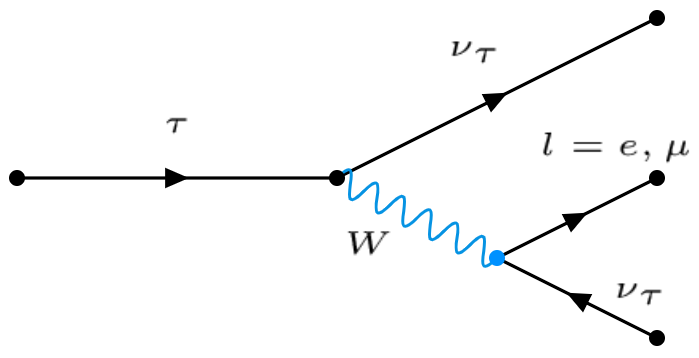
\includegraphics[width=0.6\textwidth]{figures/Fig1}
	\caption{Tau leptonic decay mode. Tau lepton is kinematically allowed to decay into muons or electrons, not that in this decay mode two neutrinos of different flavour are produced.}
	\label{Fig1}
\end{figure}
\begin{figure}[h]
	\centering
	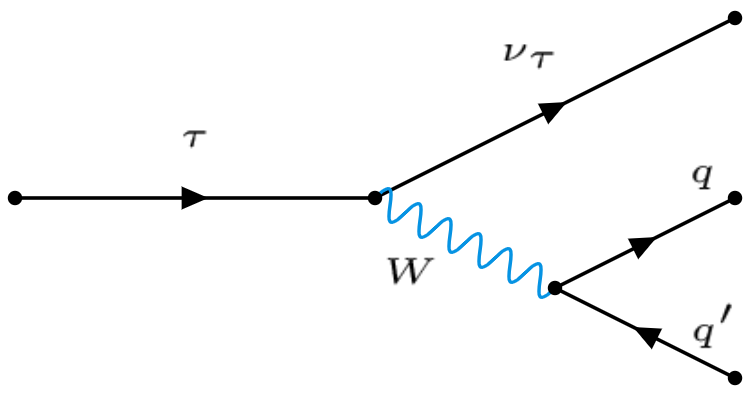
\includegraphics[width=0.6\textwidth]{figures/Fig2}
	\caption{Tau hadronic decay mode. Tau lepton is kinematically allowed only to decay into hadrons containing up, down and strange quarks. This results on final states containing multiple pions or kaons \cite{Davier_2006}.}
	\label{Fig2}
\end{figure}
Naively, if we were to estimate the branching fraction for hadronic and leptonic tau decay modes, defined as:
\begin{equation}
	\beta(\tau\to X\nu_\tau)=\frac{\Gamma(\tau\to X\nu_\tau)}{\Gamma_{\text{tot}}},
\end{equation}
where X could be any group of leptons or hadrons and $\Gamma_{\text{tot}}$ is the total decay width for the tau, we could argue that the contribution from the hadronic decays triples the contribution for one of the leptonic modes. This is because in any hadronic decay, we would have to count 3 different diagrams, like the one in Fig.\ref{Fig2} because of the 3 colour possibility for the quarks.

Thus, 
\begin{align}
\beta(\tau\to l\nu_l\nu_\tau)\approx 20\%& \hspace{1cm}l=e,\mu;
\\
\beta(\tau\to X\nu_\tau)\approx 60\%& \hspace{1cm} X=\text{hadrons+neutrinos}.
\end{align}
In fact, this naive estimation is not bad. Actual values for the leptonic branching ratios are \cite{PhysRevD.98.030001}:
\begin{align}
\beta(\tau\to e\nu_e\nu_\tau)&=17.82\pm 0.04\%
\label{eq6}
\\
\beta(\tau\to \mu\nu_\mu\nu_\tau)&=17.39\pm 0.04\%,
\end{align}
the small difference is due to the mass difference between the muon and the electron.

On the other hand, the hadronic decays of the tau are more varied and can contain much more particles in the final states. The vast majority of hadronic tau decays have charged or neutral pions in the final states, but more exotic decays including kaons also happen. Branching fractions for the most important tau hadronic decays are showed in Table \ref{Table1}.
\begin{table}[]
	\centering
\begin{tabular}{|c|c|}
	\hline
	Decay mode                     & Branching fraction \\ \hline
	$\pi^\pm \nu_\tau$             & 11.1 \%            \\ \hline
	$\pi^\pm \pi^0 \nu_\tau$       & 25.4\%             \\ \hline
	$\pi^\pm \geq 2\pi^0 \nu_\tau$ & 9.1\%               \\ \hline
	$3\pi^\pm \nu_\tau$            & 9.1\%               \\ \hline
	$3\pi^\pm \geq 1\pi^0 \nu_\tau$& 4.6\%               \\ \hline
	others						   & 5.5\%               \\ \hline
\end{tabular}
	\caption{Tau hadronic decay modes branching fractions.}
	\label{Table1}
\end{table}
\section{Lepton Universality}\label{chap2sec2}
The SM predicts that all charged leptons $(e,\mu,\tau)$ interact via the electromagnetic and weak forces and explains that this interactions can be seen as the interchange of \textit{vector bosons}, the photon $(\gamma)$ and the W and Z bosons respectively. Specifically, in the SM the form of the interaction does not depend on the lepton generation. This feature of the SM is called \textit{lepton universality} and it can be understood as that physics processes for electrons, muons and taus are almost identical copies of each other (although some small discrepancies arise from the fact that lepton masses are different and extrictly speaking lepton universality is not a exact symmetry). 

For instance, tau leptonic decay widths present a great opportunity to test lepton universality hypothesis. If we start considering muon decay, at low energies we can consider this process to be a point like interaction well described by Fermi theory \cite{FermiTheory}. In this case, if we approximate the electron and neutrinos as being massless particles, a dimensionally correct expression for the width will be of the form:
\begin{equation}
	\Gamma(\mu\to e+\nu_e +\nu_\mu)=KG_{F}^{2}m_{\mu}^{5},
\end{equation} 
where $G_F=1.1666\times 10^{-5} \text{ GeV}^{-2}$ is the Fermi coupling constant and $K$ is a constant that depends on the form of the interaction. If we assume that lepton universality holds, the respective widths for the tau leptonic decay modes, will have the form:
\begin{align}
\Gamma(\tau\to e+\nu_e +\nu_\tau)&=KG_{F}^{2}m_{\tau}^{5},
\\
\Gamma(\tau\to \mu+\nu_\mu +\nu_\tau)&=\Gamma(\tau\to e+\nu_e +\nu_\tau),
\end{align}  
and this explains why to a good approximation leptonic branching fractions for tau decay are equal. Moreover, we can obtain a relation between tau and muon lifetimes. We know that,
\begin{equation}
	\tau_l=\frac{1}{\Gamma_\text{Tot}}=\frac{\beta(l\to e\nu_e \nu_l)}{\Gamma(l\to e\nu_e \nu_l)},
	\label{eq11}
\end{equation}
also that $\beta(\mu\to e\nu_e \nu_\mu)=1$ and taking into account eq.(\ref{eq6}) we can take the ratio between eq.(\ref{eq11}) for $l=\tau ,\mu$ to obtain:
\begin{equation}
\frac{\tau_\tau}{\tau_\mu}=\frac{\beta(\tau\to e\nu_e \nu_\tau)}{\beta(\mu\to e\nu_e \nu_\mu)}\left(\frac{m_\mu}{m_\tau}\right)^5=(1.328\pm 0.004)\times 10^{-7}.
\end{equation}
This is consistent with the experimental lifetimes ratio of $(1.3227\pm 0.0005)\times10^{-7}$. This agreement on lifetimes that differ on 7 orders of magnitude is a good proof that lepton universality holds on W decays at the tau mass scale.

Very precise test of LU have been done by $e^-e^+$ colliders (LEP1, SLC and LEP2). Measurements of the ratios between the leptonic decay widths of the Z boson have been performed and are consistent with the SM \cite{ALEPH:2005ab}:
\begin{align}
	\frac{\Gamma(Z\to\mu^+\mu^-)}{\Gamma(Z\to e^+e^-)}=1.0009\pm 0.0028,
	\\
	\frac{\Gamma(Z\to\tau^+\tau^-)}{\Gamma(Z\to e^+e^-)}=1.0019\pm 0.0032.
\end{align}
LU has also been tested in W boson decays, a combination of measurements made by different experiments of the branching fractions between the first two families of leptons are consistent with SM predictions \cite{Pich:2013lsa}:
\begin{equation}
\frac{\beta(W^-\to e^-\bar{\nu_e})}{\beta(W-\to \mu^-\bar{\nu_\mu})}=1.004\pm 0.008.
\end{equation}
But measurements including the third lepton family, apart from being less precise due to the more challenging reconstruction of the $\tau$ lepton final states are in tension with SM \cite{Schael:2013ita}:
\begin{align}
\frac{\Gamma(W^-\to\tau^-\bar{\nu_\tau})}{\Gamma(W^-\to e^-\bar{\nu_e})}=1.063\pm 0.027,
\\
\frac{\Gamma(W^-\to\tau^-\bar{\nu_\tau})}{\Gamma(W^-\to \mu^-\bar{\nu_\mu})}=1.070\pm 0.026.
\end{align}
This results show that LU between the two first lepton family holds with a precision of 0.3\% and 0.8\% in Z and W decays respectively. Constraints between the third and the other two generations of leptons are of similar precision on Z boson decays (0.3\%), but ten times worse for W boson decays (3\%) and somewhat in tension with SM prediction. An example of this is a measurement exhibiting a tension of 2.6 $\sigma$ from the SM expectation \cite{Schael:2013ita}:
\begin{equation}
	\frac{2\Gamma(W^-\to\tau^-\bar{\nu_\tau})}{\Gamma(W^-\to e^-\bar{\nu_e})+\Gamma(W^-\to \mu^-\bar{\nu_\mu})}=1.066\pm 0.025.
\end{equation}  


Furthermore, measurements from LHCb, BaBar and Belle experiments have shown consistent deviations from the SM predictions \cite{Ciezarek_2017}. This experiments have independently measured a deviation on $\bar{B}$ meson semi-leptonic branching ratios, specifically:
\begin{align}
	R_D&=\frac{\beta(\bar{B}\to D\tau^-\bar{\nu}_\tau)}{\beta(\bar{B}\to De^-\bar{\nu}_e)}
	\\
	R_{D^\star}&=\frac{\beta(\bar{B}\to D^\star\tau^-\bar{\nu}_\tau)}{\beta(\bar{B}\to D^\star e^-\bar{\nu}_e)}.
\end{align}
The combined results for the different experiments are shown in Fig.\ref{Fig3} . These measurements represent a 3.08 $\sigma$
 deviation from the SM predictions, but even tough they represent a hint of new physics, these results have to be taken with care since at this point it could be that systematic uncertainties are being underestimated or statistical deviations are larger than expected. In this matters, future analysis from experiments like LHCb and Belle with larger available datasets will be very important to untangle this situation.
 \begin{figure}[h]
 	\centering
 	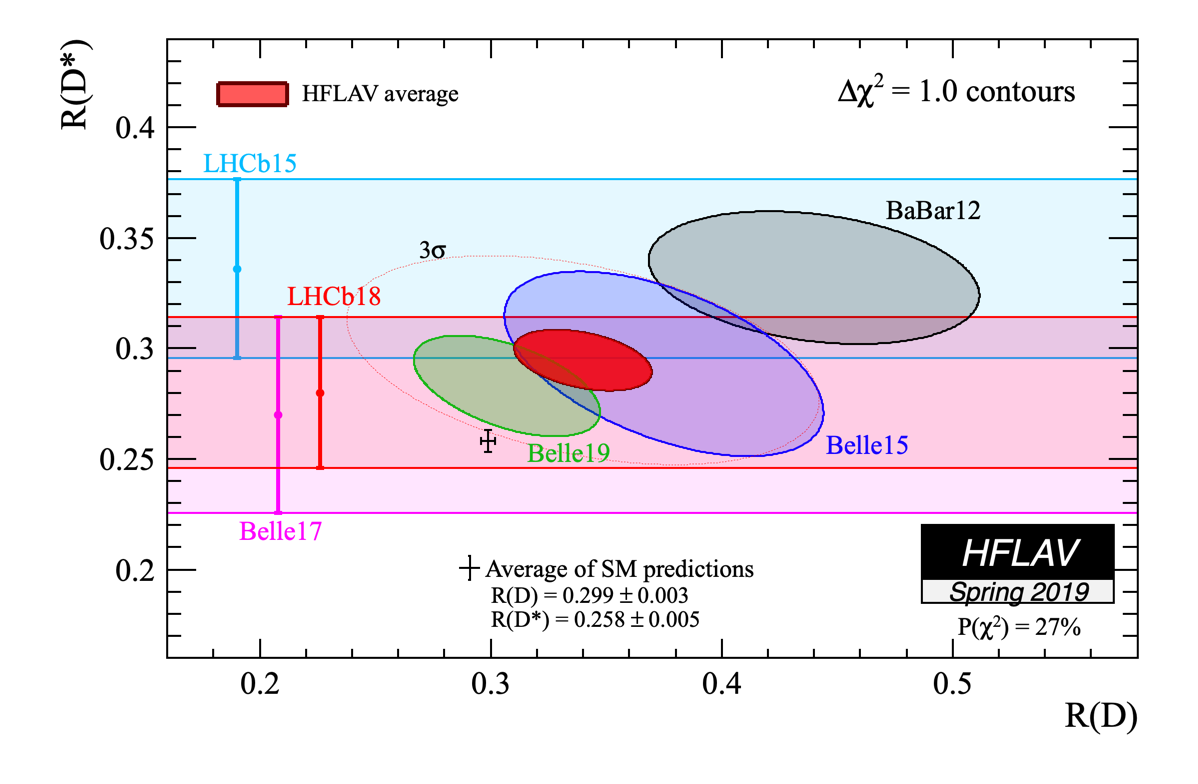
\includegraphics[width=0.7\textwidth]{figures/Fig3}
 	\caption{Combined results from BABAR,Belle and LHCb with 1-$\sigma$ contour. The average calculated by the Heavy Flavour Averaging Group \cite{HFAG}  is compared with the SM predictions.}
 	\label{Fig3}
 \end{figure}